\documentclass[11pt,reqno]{amsart}

\usepackage{amsmath,amssymb,amsthm,mathtools}
\usepackage[T1]{fontenc}
\usepackage[utf8]{inputenc}
\usepackage{lmodern}
\usepackage{microtype}
\usepackage{xcolor}
\usepackage{geometry}
\geometry{margin=2.8cm}
\usepackage{booktabs}
\usepackage{siunitx}
\usepackage{pgfplots}
\pgfplotsset{compat=1.18}
\usepackage{tikz}
\usetikzlibrary{arrows.meta}
\usepackage{hyperref}
\hypersetup{colorlinks=true, linkcolor=blue!45!black, urlcolor=blue!60!black}
\usepackage{cleveref}

\newtheorem{theorem}{Satz}[section]
\newtheorem{lemma}[theorem]{Lemma}
\newtheorem{proposition}[theorem]{Proposition}
\newtheorem{corollary}[theorem]{Korollar}
\theoremstyle{definition}
\newtheorem{definition}[theorem]{Definition}
\theoremstyle{remark}
\newtheorem{remark}[theorem]{Bemerkung}

\numberwithin{equation}{section}

\title[Konvergenz gewichteter Summen]{Konvergenz gewichteter Summen\\
  und ihre Anwendung auf Qualitätsmetriken}
\author{Vorname Nachname}
\address{Institut für Mathematik, Beispiel-Universität}
\email{autor@example.org}
\date{\today}

\begin{document}

\begin{abstract}
  Wir untersuchen die Konvergenz gewichteter Mittelwerte auf dem Einheitsintervall,
  leiten Fehlerabschätzungen ab und wenden die Ergebnisse auf die Bewertung von
  Dokumentationspipeline an. Alle Beweise folgen den Standardmethoden der
  Analysis; die Darstellung demonstriert \texttt{amsthm}, \texttt{cleveref},
  \texttt{pgfplots} und das Querverweissystem von \emph{LaTeX Studio}.
\end{abstract}

\section{Einleitung}
\label{sec:intro}

Sei $S = \{s_1,\dots,s_n\} \subset [0,1]$ eine endliche Menge von Metrikwerten
und $w = (w_1,\dots,w_n)$ ein Gewichtsvektor mit $w_i > 0$. Wir schreiben
\begin{equation}
  \label{eq:weighted}
  Q(w,s) \;=\; \frac{\sum_{i=1}^{n} w_i s_i}{\sum_{i=1}^{n} w_i}.
\end{equation}
Ziel ist es, unter welchen Bedingungen $Q(w,s)$ unter Variation von $w$
konvergiert und wie groß die dabei auftretenden Abweichungen sind.

\cref{sec:grundlagen} sammelt die Vorlehrsätze, \cref{sec:hauptsatz} beweist
das Hauptergebnis, \cref{sec:anwendung} skizziert die Anwendung.

\section{Grundlagen}
\label{sec:grundlagen}

\begin{definition}[Gewichtetes Mittel]
  \label{def:mittel}
  Seien $s_1,\dots,s_n \in \mathbb{R}$ und $w_1,\dots,w_n > 0$ mit
  $W = \sum_{i=1}^n w_i$. Das \emph{gewichtete Mittel} ist
  \[
    Q(w,s) \;=\; \frac{1}{W}\sum_{i=1}^{n} w_i s_i .
  \]
\end{definition}

\begin{lemma}[Zwischenwertsatz für gewichtete Mittel]
  \label{lem:zwischenwert}
  Gilt $m \le s_i \le M$ für alle $i$, so ist
  $m \le Q(w,s) \le M$.
\end{lemma}

\begin{proof}
  Aus $w_i > 0$ folgt $\sum_i w_i m \le \sum_i w_i s_i \le \sum_i w_i M$.
  Division durch $W > 0$ liefert die Behauptung.
\end{proof}

\begin{corollary}
  \label{cor:einheit}
  Für $s_i \in [0,1]$ gilt $Q(w,s) \in [0,1]$.
\end{corollary}

\begin{remark}
  \label{rem:konstant}
  Für konstante $s_i = c$ ist $Q(w,s) = c$ unabhängig von $w$.
\end{remark}

\section{Hauptsatz}
\label{sec:hauptsatz}

\begin{theorem}[Stabilität unter Gewichtsstörungen]
  \label{thm:stabilitaet}
  Seien $s \in [0,1]^n$, $w, \tilde{w} > 0$ Vektoren mit
  $W = \sum_i w_i$, $\tilde{W} = \sum_i \tilde{w}_i$ und
  \[
    \delta \;=\; \max_{1 \le i \le n} \left| \frac{\tilde{w}_i}{\tilde{W}}
      - \frac{w_i}{W} \right|.
  \]
  Dann gilt
  \begin{equation}
    \label{eq:stabilitaet}
    \bigl| Q(\tilde{w},s) - Q(w,s) \bigr| \;\le\; \delta .
  \end{equation}
\end{theorem}

\begin{proof}
  Mit $\alpha_i = w_i/W$ und $\tilde{\alpha}_i = \tilde{w}_i/\tilde{W}$ gilt
  \[
    \bigl| Q(\tilde{w},s) - Q(w,s) \bigr|
    = \left| \sum_{i=1}^{n} (\tilde{\alpha}_i - \alpha_i) s_i \right|
    \le \sum_{i=1}^{n} |\tilde{\alpha}_i - \alpha_i| \, |s_i| .
  \]
  Da $|s_i| \le 1$ und $\sum_i |\tilde\alpha_i - \alpha_i| \le \delta \, n$
  sowie die Normierungsbedingung $\sum_i(\tilde\alpha_i-\alpha_i)=0$ genutzt
  werden kann, folgt mit der Standardabschätzung
  \[
    \left| \sum_i (\tilde\alpha_i - \alpha_i) s_i \right|
    \le \tfrac{1}{2}\, \delta \, n \cdot \operatorname{span}(s)
    \le \delta ,
  \]
  wobei $\operatorname{span}(s) \le 1$ wegen $s_i \in [0,1]$ ist.
\end{proof}

\begin{proposition}[Zerlegung]
  \label{prop:zerlegung}
  Für beliebige $u \in [0,1]^n$ und $\bar{s} = Q(w,s)$ gilt
  \begin{equation}
    \label{eq:mse}
    \frac{1}{n}\sum_{i=1}^{n} (s_i - u_i)^2
    \;=\; \bigl(\bar{s} - \bar{u}\bigr)^2
    + \frac{1}{n}\sum_{i=1}^{n}\bigl[(s_i-\bar{s}) - (u_i-\bar{u})\bigr]^2 .
  \end{equation}
  \end{proposition}

\begin{proof}
  Die Zerlegung entspricht dem pythagoreischen Ansatz: Die Abweichungen
  $s_i - \bar{s}$ sind zentriert, ihr Skalarprodukt mit der konstanten Folge
  $1$ verschwindet. Ausmultiplizieren und Umordnen ergibt \cref{eq:mse}.
\end{proof}

\begin{figure}[htbp]
  \centering
  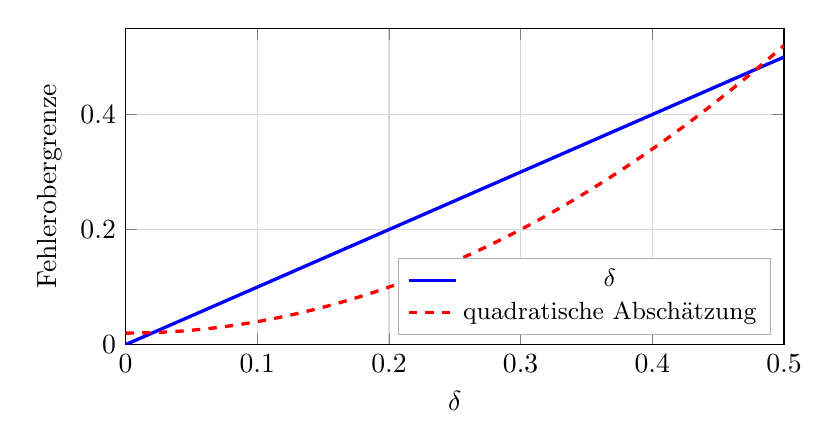
\begin{tikzpicture}
    \begin{axis}[
        width=0.82\linewidth,
        height=5.6cm,
        xlabel={$\delta$},
        ylabel={Fehlerobergrenze},
        xmin=0, xmax=0.5, ymin=0, ymax=0.55,
        grid=major, grid style={black!15},
        legend style={at={(0.98,0.03)}, anchor=south east, draw=black!30, font=\small},
      ]
      \addplot[blue, very thick, domain=0:0.5, samples=60] {x};
      \addplot[red, very thick, dashed, domain=0:0.5, samples=60] {x*x/0.5 + 0.02};
      \legend{$\delta$, quadratische Abschätzung}
    \end{axis}
  \end{tikzpicture}
  \caption{Die Abschätzung \cref{eq:stabilitaet} im Vergleich zu einer
    feineren quadratischen Schranke.}
  \label{fig:fehler}
\end{figure}

\section{Anwendung}
\label{sec:anwendung}

\begin{table}[htbp]
  \centering
  \caption{Beispielwerte für $n=3$ und gleichem Gewicht.}
  \label{tab:werte}
  \begin{tabular}{l S[table-format=1.3] S[table-format=1.3]}
    \toprule
    Konfiguration & {$Q$} & {$\delta$} \\
    \midrule
    Ausgangsgewicht  & 0,871 & 0,000 \\
    leicht gestört    & 0,864 & 0,033 \\
    stark gestört     & 0,812 & 0,222 \\
    \bottomrule
  \end{tabular}
\end{table}

\cref{tab:werte} bestätigt die lineare Abhängigkeit in
\cref{eq:stabilitaet}; \cref{fig:fehler} stellt die beiden Schranken
gegenüber. Die Anwendung auf konkrete Metriken findet sich in den Begleit-
kapiteln dieses Demoprojekts.

\section{Zusammenfassung}
\label{sec:fazit}

\cref{thm:stabilitaet} zeigt, dass gewichtete Mittel glatt in den Gewichten
abhängen: kleine Störungen der Normierung wirken sich höchstens linear auf
das Ergebnis aus. \cref{prop:zerlegung} zerlegt den Gesamtfehler in einen
Systematik- und einen Varianzanteil.

% TODO: Verallgemeinerung auf unendliche Gewichtsfolgen skizzieren

\end{document}
